\begin{figure}[H]
	\begin{center}
		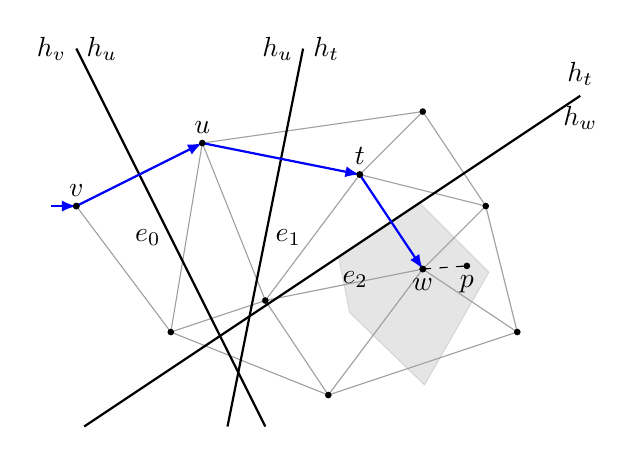
\begin{tikzpicture}[scale=0.4]
		%\draw [<->,thick] (0,10) node (yaxis) [left] {}
		%|- (15,0) node (xaxis) [below] {};
		
		%VORONOI
%		\draw [-,gray!50] ( 5.6764, 5.9706) -- ( 4.9545, 6.0909);
%		\draw [-,gray!50] ( 5.6764, 5.9706) -- ( 8.1956, 6.9783);
%		\draw [-,gray!50] (10.3235, 5.3824) -- ( 8.1956, 6.9783);
%		\draw [-,gray!50] (10.3235, 5.3824) -- (10.6765, 3.6176);
%		\draw [-,gray!50] ( 7.2272, 1.3182) -- (10.6765, 3.6176);
%		\draw [-,gray!50] ( 7.2272, 1.3182) -- ( 5.6764, 5.9706);
%		\draw [-,gray!50] (13.0556, 1.3182) -- (10.6765, 3.6176);
%		\draw [-,gray!50] (13.0556, 1.3182) -- (15.1000, 4.9000);
%		\draw [-,gray!50] (12.9000, 7.1000) -- (15.1000, 4.9000);
%		\draw [-,gray!50] (12.9000, 7.1000) -- (10.3235, 5.3824);
%		\draw [-,gray!50] (12.9000, 7.1000) -- (13.1000, 7.9000);
%		\draw [-,gray!50] ( 9.1667,11.8333) -- (13.1000, 7.9000);
%		%\draw [-,gray!50] ( 9.1667,11.8333) -- ( 8.1956, 6.9783);
%		%VORONOI EXTENDED
%		\draw [-,gray!50] ( 4.9545, 6.0909) -- (2 , 12);
%		\draw [-,gray!50] ( 4.9545, 6.0909) -- (0, 2.375);
%		\draw [-,gray!50] ( 7.2272, 1.3182) -- ( 6.7, 0);
%		\draw [-,gray!50] (13.0556, 1.3182) -- (13.6667, 0);
%		\draw [-,gray!50] (15.1000, 4.9000) -- (18, 5.625);
%		\draw [-,gray!50] (13.1000, 7.9000) -- (18, 11.1667);
%		\draw [-,gray!50] ( 9.1667,11.8333) -- ( 9.1429, 12);
		
		\filldraw[fill=black, opacity=0.1] 	(10.3235, 5.3824) -- (10.6765, 3.6176) --
											(13.0556, 1.3182) -- (15.1000, 4.9000) --
											(12.9000, 7.1000) -- cycle;
		
		%DELAUNAY
		\draw [-,gray!75] ( 2,7) -- ( 6,9);
		\draw [-,gray!75] ( 6,9) -- ( 5,3);
		\draw [-,gray!75] ( 5,3) -- ( 2,7);
		\draw [-,gray!75] ( 6,9) -- ( 8,4);
		\draw [-,gray!75] (10,1) -- ( 8,4);
		\draw [-,gray!75] ( 5,3) -- (10,1);
		\draw [-,gray!75] ( 8,4) -- ( 5,3);
		\draw [-,gray!75] ( 8,4) -- (11,8);
		\draw [-,gray!75] (11,8) -- (6,9);
		\draw [-,gray!75] ( 6,9) -- (13,10);
		\draw [-,gray!75] (11,8) -- (13,10);
		\draw [-,gray!75] (15,7) -- (13,10);
		\draw [-,gray!75] (16,3) -- (15,7);
		\draw [-,gray!75] (16,3) -- (10,1);
		\draw [-,gray!75] (16,3) -- (13,5);
		\draw [-,gray!75] (13,5) -- (15,7);
		\draw [-,gray!75] (13,5) -- (10,1);
		\draw [-,gray!75] (13,5) -- (8,4);
		\draw [-,gray!75] (13,5) -- (11,8);
		\draw [-,gray!75] (15,7) -- (11,8);
		
		
		%POINTS
		
		\fill ( 2, 7) circle (3pt);
		\fill ( 5, 3) circle (3pt);
		\fill ( 8, 4) circle (3pt);
		\fill (10, 1) circle (3pt);
		\fill (11, 8) circle (3pt);
		\fill (13, 5) circle (3pt);
		\fill (13,10) circle (3pt);
		\fill (15, 7) circle (3pt);
		\fill (16, 3) circle (3pt);
		
		%EDGE E
		\draw [-,thick] ( 8,0)		-- node[left]{$e_0$} ( 2, 12)	node[left]		{$h_v$} node[right]{$h_u$};
		\draw [-,thick] ( 6.8,0)	-- node[right]{$e_1$} (9.2,12)	node[left] 		{$h_u$} node[right]{$h_t$};
		\draw [-,thick] ( 2.25,0)	-- node[below right]{$e_2$} (18,10.5)	node[above]{$h_t$} node[below]{$h_w$};
		
		
		\draw [-,dashed]( 13,5) -- ( 14.4, 5.1);
		\draw [->,>=latex,thick,blue]( 1.2,7) -- (  2,7);
		\draw [->,>=latex,thick,blue]( 2,7) -- (  6,9);
		\draw [->,>=latex,thick,blue]( 6,9) -- ( 11, 8);
		\draw [->,>=latex,thick,blue](11,8) -- ( 13, 5);
		\fill (14.4, 5.1) circle (3pt) node[anchor=north]{$p$};
		\fill ( 2, 7)     circle (3pt) node[anchor=south]{$v$};
		\fill ( 6, 9)     circle (3pt) node[anchor=south]{$u$};
		\fill (11, 8)     circle (3pt) node[anchor=south]{$t$};
		\fill (13, 5)     circle (3pt) node[anchor=north]{$w$};
		
		\end{tikzpicture}
	\end{center}
	\caption{Example of the Greedy Routing Algorithm}
	\label{fig:gr1}
\end{figure}